\documentclass[aspectratio=169,10pt]{beamer}
\usepackage[T1]{fontenc}
\usepackage{amsmath,amssymb,amsfonts}
\usepackage{bm}
\usepackage{tikz}
\usepackage{xcolor}
\usetikzlibrary{arrows.meta,positioning,shapes,calc}

\definecolor{parchment}{HTML}{F4E8C8}
\definecolor{paper}{HTML}{FAF1D8}
\definecolor{ink}{HTML}{1A1A1A}
\definecolor{inkgray}{HTML}{5A5A5A}
\definecolor{accentred}{HTML}{8B1A1A}
\definecolor{accentgreen}{HTML}{2D5F2C}
\definecolor{accentblue}{HTML}{1F4E79}
\definecolor{redbg}{HTML}{F7E0DE}
\definecolor{grnbg}{HTML}{E0EBDC}
\definecolor{blubg}{HTML}{DDE6EF}
\definecolor{labelbg}{HTML}{EFE0B0}

\usefonttheme{serif}
\setbeamercolor{background canvas}{bg=parchment}
\setbeamercolor{normal text}{fg=ink}
\setbeamercolor{structure}{fg=ink}
\setbeamercolor{frametitle}{fg=ink,bg=parchment}
\setbeamercolor{title}{fg=ink}
\setbeamercolor{itemize item}{fg=ink}
\setbeamercolor{itemize subitem}{fg=ink}
\setbeamercolor{item}{fg=ink}
\setbeamercolor{caption name}{fg=ink}
\setbeamertemplate{navigation symbols}{}
\setbeamertemplate{itemize item}{\textbullet}

\setbeamertemplate{frametitle}{%
  \vspace{0.30em}%
  \begin{center}%
    {\bfseries\Large\insertframetitle\par}%
    \vspace{0.28em}%
    {\color{ink}\rule{0.86\paperwidth}{0.4pt}}%
  \end{center}%
  \vspace{0.10em}%
}
\setbeamertemplate{footline}{%
  \hbox to \paperwidth{\hfil\itshape\small\insertframenumber\hspace{0.7em}}%
  \vspace{0.35em}%
}

\newcommand{\vY}{\bm{Y}}
\newcommand{\vy}{\bm{y}}
\newcommand{\vA}{\bm{A}}
\newcommand{\vB}{\bm{B}}
\newcommand{\valpha}{\bm{\alpha}}
\newcommand{\vn}{\bm{n}}
\newcommand{\vs}{\bm{s}}
\newcommand{\vW}{\bm{W}}
\newcommand{\T}{^{\mathsf T}}
\newcommand{\Hh}{^{\mathsf H}}
\newcommand{\norm}[1]{\left\lVert #1\right\rVert}
\DeclareMathOperator*{\argmin}{arg\,min}

\tikzset{
  flowbox/.style={draw=ink,fill=paper,line width=0.6pt,
                  minimum width=2.5cm,minimum height=1.0cm,
                  align=center,font=\small\bfseries,inner sep=4pt},
  smallbox/.style={draw=ink,fill=paper,line width=0.4pt,
                   minimum width=0.7cm,minimum height=0.55cm,
                   inner sep=2pt,align=center,font=\footnotesize\itshape},
  method/.style={draw=accentgreen,fill=grnbg,line width=1.0pt,
                 align=center,font=\small\bfseries,inner sep=6pt},
  issue/.style={draw=accentred,fill=redbg,line width=1.0pt,
                align=center,font=\small\bfseries,inner sep=6pt},
  idea/.style={draw=accentblue,fill=blubg,line width=1.0pt,
               align=center,font=\small\bfseries,inner sep=6pt},
  flowarr/.style={-{Stealth[length=2.5mm,width=2mm]},line width=0.7pt},
  softarr/.style={-{Stealth[length=2mm,width=1.6mm]},line width=0.5pt,color=inkgray}
}

\newcommand{\bottomnote}[1]{%
  \begin{center}{\itshape\small #1}\end{center}}

\newcommand{\papercover}[4]{%
  \begin{frame}[plain]
    \vfill
    \begin{center}
      {\bfseries\Huge #1\par}
      \vspace{0.8cm}
      {\Large #2\par}
      \vspace{0.35cm}
      {\itshape\large\color{inkgray}#3\par}
      \vspace{0.55cm}
      {\small\texttt{\detokenize{#4}}\par}
    \end{center}
    \vfill
  \end{frame}}

\newcommand{\twocolmodel}[4]{%
  \begin{columns}[T,onlytextwidth]
    \begin{column}{0.48\textwidth}#1\end{column}
    \begin{column}{0.48\textwidth}#2\end{column}
  \end{columns}
  \bottomnote{#3\\#4}}


\begin{document}

\papercover
  {Clustered Channel Adaptation}
  {Zhaohui Wang, Shengli Zhou, Preisig, Pattipati, and Willett}
  {IEEE Transactions on Signal Processing, 2012}
  {clustered_channel_adaptation_ofdm_uwa.pdf}

\begin{frame}{1. Core Problem}
\twocolmodel{
  \begin{itemize}\setlength{\itemsep}{0.45em}
    \item UWA paths are sparse, but they are not isolated one by one.
    \item Paths form clusters from refraction, surface bounce, and bottom bounce routes.
    \item Different clusters evolve differently across OFDM blocks.
  \end{itemize}
}{
  \[
    \mathcal S
    =
    \mathcal C_1\cup\mathcal C_2\cup\cdots\cup\mathcal C_G
  \]
  \[
    \Delta_g=(\Delta a_g,\Delta \tau_g,\Delta \alpha_g)
  \]
}{
  The paper adds memory across blocks without forcing the whole channel to move as one object.
}{
  Cluster-level variation is the compromise between dense re-estimation and one global update.
}
\end{frame}

\begin{frame}{2. Adaptation Model}
\begin{center}
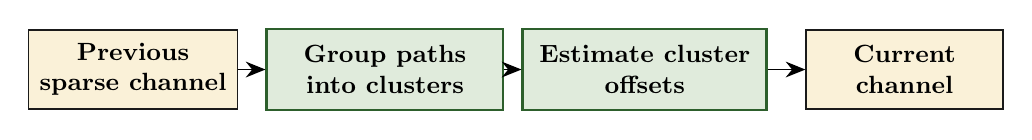
\begin{tikzpicture}[x=1cm,y=1cm]
  \node[flowbox] (prev) at (-5.0,0) {Previous\\sparse channel};
  \node[method,minimum width=3.0cm] (cluster) at (-1.8,0) {Group paths\\into clusters};
  \node[method,minimum width=3.0cm] (offset) at (1.5,0) {Estimate cluster\\offsets};
  \node[flowbox] (curr) at (4.8,0) {Current\\channel};
  \draw[flowarr] (prev) -- (cluster);
  \draw[flowarr] (cluster) -- (offset);
  \draw[flowarr] (offset) -- (curr);
\end{tikzpicture}
\end{center}
\[
  \widehat{\Delta}_g
  =
  \argmin_{\Delta_g}
  \norm{\vy_{\mathcal P}^{(b)}
  -\vA_{\mathcal P}\big(\mathcal C_g+\Delta_g\big)\valpha_g}_2^2
\]
\bottomnote{Use last block's channel as a structured prior, then let each cluster drift on its own.}
\end{frame}

\begin{frame}{3. Hybrid Estimator}
\begin{itemize}\setlength{\itemsep}{0.48em}
  \item Keep sparse path knowledge from the previous OFDM block.
  \item Estimate cluster-specific amplitude, delay, and Doppler changes from current pilots.
  \item Combine adapted prior paths with new pilot evidence.
  \item Outperform purely block-by-block pilot estimation when coherence exists.
\end{itemize}
\bottomnote{The estimator uses memory, but it avoids the fragile assumption that every path shares the same motion.}
\end{frame}

\begin{frame}{4. JUNA Connection}
\begin{itemize}\setlength{\itemsep}{0.5em}
  \item JUNA can regularize branch coefficients by cluster:
  \[
    \bm c_{kq}^{(b)}
    \approx
    \bm c_{kq}^{(b-1)}+\text{cluster drift}.
  \]
  \item Cluster identity is a discrete structure; estimate it explicitly or by candidates.
  \item Low-dimensional cluster offsets are reasonable continuous refinement variables.
  \item This paper is a strong guide for temporal smoothing in a self-calibrating receiver.
\end{itemize}
\end{frame}

\end{document}
